\chapter{Straight list} \label{ch:straight-list}

We have a video, since videos can be simplified as frames, or images, in sequence. Our access to all elements mustn't be restricted, so we can't use \nameref{pt:one}. 

One solution would be to use arrays, but that is where a problem might emerge. The array would save each frame inside it in continuous memory, so if a one hour video consists of \(30_{fps} \times 60_{sec} \times 60_{min} = 108,000\) frames in total, and each frame is an image with \(4_{RGBA} \times 1920 \times 1080 = 8,294,400\) bytes (8.3MB), the total is \(108,000_{frames} \times 8,294,400_{bytes} = 895,795,200,000\) or \textasciitilde 896GB, wait, what, i-its actually this much? Thankfully we have video-compression. Now, it is pointless to use an array, but if we have a linked list with one 8.3MB (plus 8 bytes for a pointer) frame each scattered throughout our memory, we could maybe at least store it in memory holes. 

Another solution is to treat each frame as a pointer and store them in an array of \(108,000_{frames} \times 8B_{pointer} = 864,000\) byte size. The frames are scattered throughout the memory if we allocate space for each separately.

Using linked lists as a linear representation for each frame in a video gives us the ability to remove (cut out) parts of the video. Another feature is inserting a set of frames at any point in the video (combine).

A straight list is a special name I came up with to describe a singly-linked acyclic list. Adding and removing frames is easiest when done from the beginning, or head. That is because the to get to any other part of the list, a saved link variable must traverse through the entire structure to reach the end. This is most similar to how the \nameref{ch:stack} adds and retrieves the last inserted element first in the fastest way possible.

\section{Implementations of a straight list}

The straight list can have either one or many forms of realizations in C, depending on how far-stretched the definition of a singly-linked acyclic list is. But all can agree that the base implementation consists of a structure called a node, which contains a value and a reference. The reference, in C a pointer, references either the next node in the list or a special reference symbolizing the end of the list (NULL). 

\begin{infobox}[title=Linux manual page - NULL(3const)]
NULL represents a null pointer constant, that is, a pointer that does not point to anything.
\end{infobox}

Other forms of lists, like in this chapter, represent lists with arrays and are more concerned with how nodes are stored inside arrays. The issues they solve center around value packing inside arrays (sparse and dense arrays), and array node order based on insertions (sequential and pseudorandom ordering). The classing linked list can also be viewed from an array perspective, since the used memory can be represented as a one-dimensional array.

\begin{figure}
    \centering
    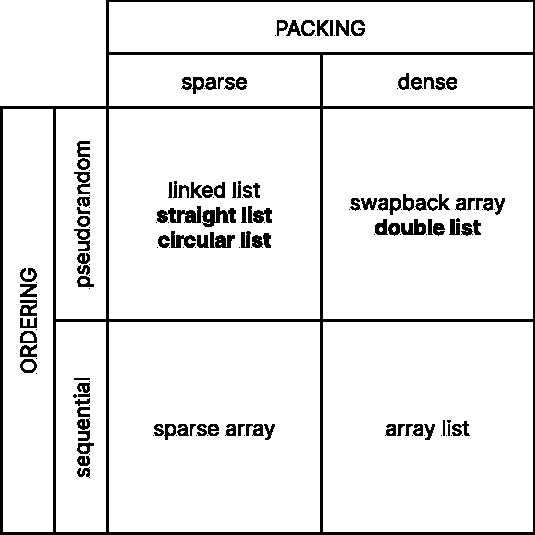
\includegraphics[width=0.7\textwidth]{figures/straight-list/list-classification.pdf}
    \caption{Classification of list-esque data structures. The ones in bold contain this part's list implementations. PACKING refers to how the data is stored inside the array - sparse means holes, dense no holes. ORDERING is based on array, not list, order relative to all memory or chunks of it.}
    \label{fig:list-classification}
\end{figure}

This chapter will only cover the classic linked list, sparse array and straight list.

\subsection{A bread of crumbs - the linked list}

The ordering of elements in a linked list (in memory) depends on the function which retrieves an uninitialized point in memory. Mostly that is done using the \texttt{malloc()}, short for [m]emory-[alloc]ation, function. Most lectures teach linked lists in C with the help of \texttt{malloc()}. With \texttt{malloc()}, memory is given to you in a way that is not guaranteed to be continuous, so the order of elements in memory is not guaranteed to be the same as the order of elements in the list. Ideally, the order of elements in memory should be the same as in the list, mainly to avoid jumping back and forth in memory, which was visited either directly or in the area. On the other hand the memory can be too far away, so visiting it and returning will simply add, spoiler alert - pointless overhead. 

The simplest solution would be to not use \texttt{malloc}. As long as the list has no references, only data, and is only being inserted into, we can use an array using \sout{\texttt{malloc()}, if the array is short, we can use \texttt{realloc()}} local memory, or even global memory!!! So what if we are just stuck with a finite array to store data, the \texttt{malloc()} school class enemy is no more. So what to do if we wanna allow element removal?

\subsection{A slice of emmental - the sparse array}

The sparse array allows element removal, but under some conditions:

\begin{enumerate}
    \item The sparse array should insert the next element rightmost to the right of the last inserted element, to preserve sequentiality.
    \item If an element is removed, the list must indicate that the place the element was saved is empty, or to be more precise, inaccessible.
\end{enumerate}

Solution number one must therefore save a count of all insertion calls, not just the current number of elements in the sparse array. This is because the next element must be inserted at the rightmost position, which is not necessarily the same as the current number of elements in the sparse array.

Solution number two has two common solutions, either a special value is used to indicate that the element is empty, or another array is used to tell where to skip to the next valid element. The first solution still forces you to check in if the memory space is valid, which can be process intensive if elements are separated by oceans of special empty values. And we loose the special value - we won' be able to use it if needed. The one point fifth solution requires another array of booleans or even bits to check if a space is empty - \texttt{true} if filled, \texttt{false} if empty. The second solution is more efficient, but requires more memory to store the second array and more logic. The empty spaces are also called holes, so if there is a hole, then why not just fill it?

